
\newthought{Problem `Dutch National Flag'} in \textit{Programming, The Derivation of Algorithms}\cite{Kaldewaij90}.\index{Fibolucci}

\vspace{10 mm}
\begin{problem}
Write a program that swaps elements of an array containing colors red, white and blue in such a way that the array's final state is in accordance with the Dutch National Flag. 
\end{problem}

\begin{marginfigure}

\includegraphics[scale=0.30]{flag.png}
\end{marginfigure}

We hope to solve this problem in linear time, going only once through the array in a loop. 


Our array is $A[0,\ldots,n)$ with 

$$
\forall i: 0 \leq i < n: A[i] \in \{ {\color{red} \squadfill}, \squad,  {\color{blue} \squadfill} \}
$$


The desired final state of the array has 3 contiguous regions: the red region, the white region and the blue region. Two indices $r$ and $w$ into the array are sufficient to show the extent of each region. We define post condition $R$

\begin{align*}
R & \equiv (\forall i: 0 \leq i < r: A[i] = {\color{red} \squadfill}) \\
  & \wedge (\forall i: r \leq i < w: A[i] = \squad) \\
  & \wedge (\forall i: w \leq i < n: A[i] = {\color{blue} \squadfill})
\end{align*}

Our loop invariant $P$ will be a relaxation\footnote{Relaxation is a common technique to derive a useful loop invariant from a post condition. A common way to do the relaxation is to introduce a variable that in the beginning completely relaxes the condition and that then gradually changes and tightens the condition to its final desired form.} of the post condition $R$. We need to introduce a new index variable $b$ to capture the notion of unprocessed region:

\begin{align*}
P & \equiv (\forall i: 0 \leq i < r: A[i] = {\color{red} \squadfill}) \\
  & \wedge (\forall i: r \leq i < w: A[i] = \squad) \\
  & \wedge (\forall i: w \leq i < b: A[i]  \text{ has not been processed yet}) \\
  & \wedge (\forall i: b \leq i < n: A[i] = {\color{blue} \squadfill})
\end{align*}

This allows us to assign values to our indices $r$, $w$ and $b$ that satisfy $P$ before the loop starts by extending the unprocessed region to be the whole array and making the red, white and blue regions empty\footnote{This is the key insight for solving the problem. Instead of having only three color regions to work with, we introduce a fourth region of unprocessed elements and we gradually shrink it. In the beginning this fourth region is the whole array and the color regions are all three empty. As the unprocessed region shrinks, the color regions start to grow in such a way that $P$ always stays true. In the end the unprocessed region is empty and the three color regions are in their final desired state thanks to $P$ always holding.}:

\begin{align*}
r & \leftarrow 0 \\
w & \leftarrow 0 \\
b & \leftarrow n
\end{align*}

Our goal now is to maintain the loop invariant $P$ while reducing the unprocessed region by processing array elements and swapping them until the unprocessed region is empty, so $b - w = 0$ or $b = w$. We then have $b = w \wedge P \Rightarrow R$. The swapping needs to happen in such a way that $P$ always holds. We also want to make progress each time through the loop, so we want $b - w$ to get smaller each time through the loop. We achieve progress by either increasing $w$ or decreasing $b$. As long as $b > w$ we go through the loop.

We will do a case analysis of the state at the region borders of processed and unprocessed regions of the array.

Let's start with a simple case: $A[w] = \squad$. Then moving $w$ one position to the right extends the white region, maintains $P$ and shrinks $b - w$, so makes progress. We write this down as one case for the loop body:

$$
\text{if } A[w] = \squad \text{ then } w \leftarrow w + 1 \text{ endif}
$$

Because we are inside the loop we know that $b > w$, so $A[b - 1]$ exists, ie $b - 1$ is a valid index position. If $A[b - 1] = {\color{blue} \squadfill}$, then we can extend the blue region to the left and thus also shrink the unprocessed region while maintaining $P$:

$$
\text{if } A[b - 1] = {\color{blue} \squadfill} \text{ then } b \leftarrow b - 1 \text{ endif}
$$

We have a couple more cases to cover.

If $A[w] = {\color{blue} \squadfill}$ then we can do our first swap: we swap $A[w]$ with $A[b-1]$ which will allow us after the swap to extend the blue region to its left as done in the previous case. As before this maintains $P$ and is progress. Let's capture this for the body of our loop:

$$
\text{if } A[w] = {\color{blue} \squadfill} \text{ then } A[w] \leftrightarrow A[b-1] \text{ ; } b \leftarrow b - 1 \text{ endif}
$$

If $A[w] = {\color{red} \squadfill}$ then we can do the following swap: we swap $A[r]$ with $A[w]$. We can then extend the red region to its right. Whatever the white region was (empty or not), it also shifts to the right by one (as a region it hasn't changed, just the first white element might have moved to be the last element of the white region if the white region was not empty):

$$
\text{if } A[w] = {\color{red} \squadfill} \text{ then } A[w] \leftrightarrow A[r] \text{ ; } r \leftarrow r + 1 \text{ ; } w \leftarrow w + 1 \text{ endif}
$$

These cases\footnote{These cases are biased towards making progress from the left to the right. One can make similar choices that cover more cases on the right border of the unprocessed region.} are sufficient to allow us to make progress while maintaining $P$. Because $b-w$ is finite and we reduce it each time through the loop, the loop will terminate. Our final program (in Go syntax) is:

\begin{lstlisting}[language=Go, frame=single]  
r := 0
w := 0
b := 0
for w < b {
   switch {
   case A[w] == White: w = w + 1
   case A[b-1] == Blue: b = b - 1
   case A[w] == Blue: swap(A[w], A[b-1]) 
                      b = b - 1
   case A[w] == Red: swap(A[w], A[r])
                     r = r + 1
                     w = w + 1
   }
}          
\end{lstlisting}

The loop invariant $P$ is maintained throughout and when the loop exits, we have $b = w$ which establishes $R$.

\begin{figure}
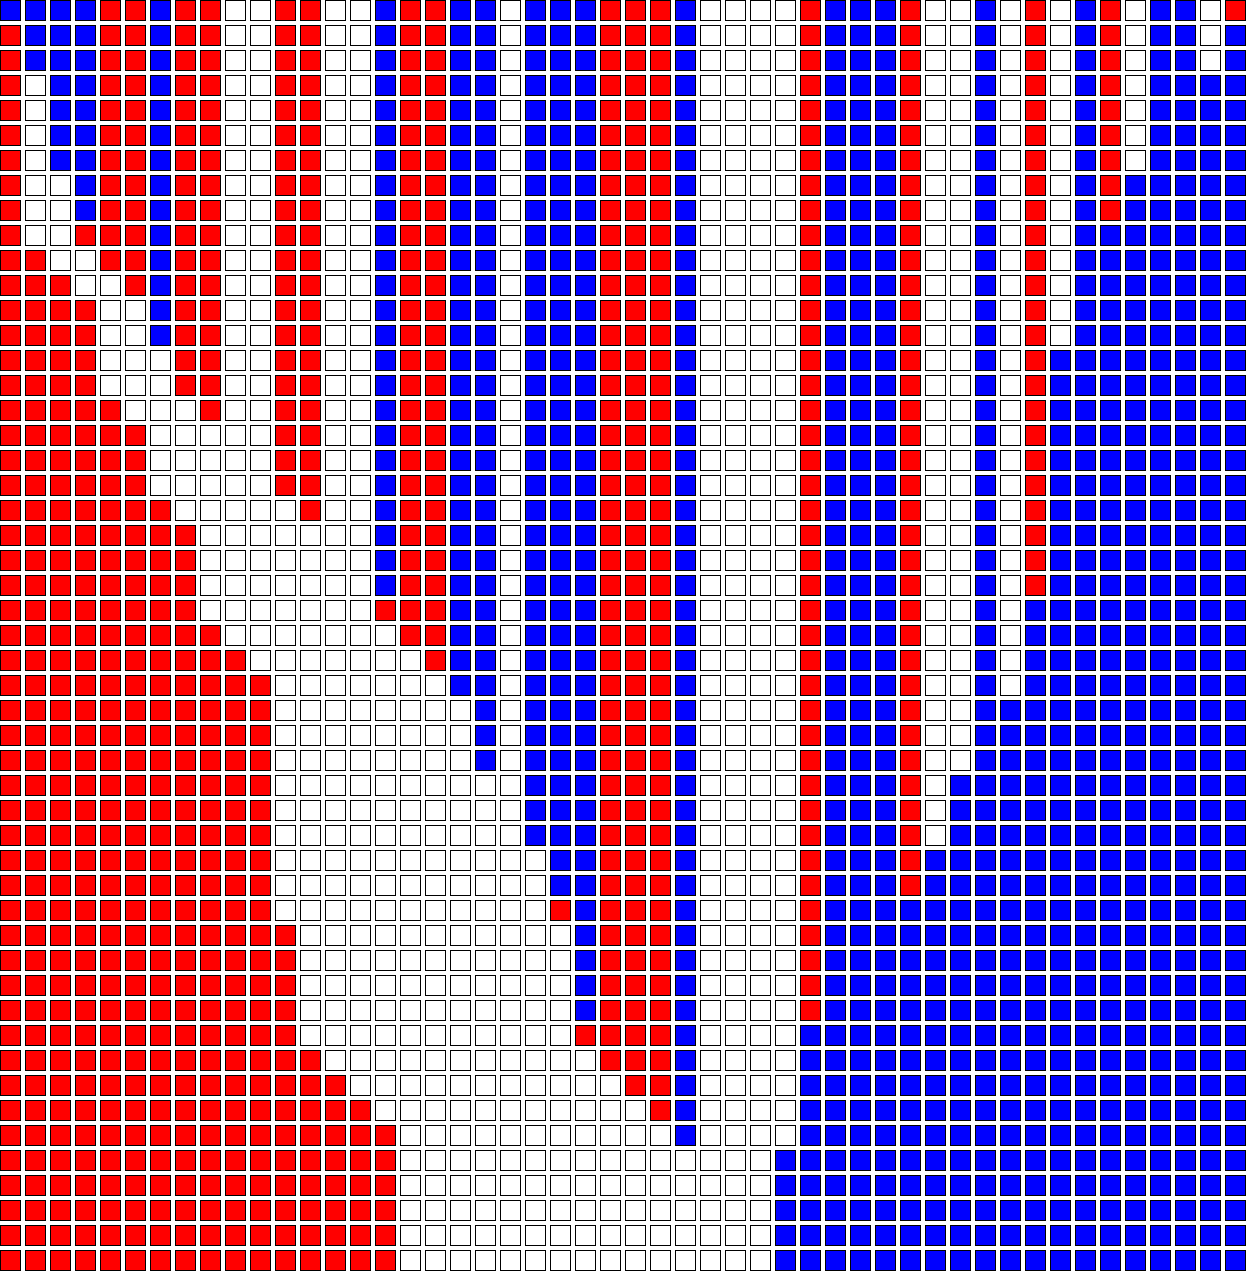
\includegraphics[scale=0.5]{largerun.pdf}
\caption{Example of processing an array. The first row is the initial state of the array. Each row below is one time through the loop. It is interesting to see that even though condition $R$ is satisfied towards the end while $b > w$, the loop still has to process elements until $b = w$, not doing any more swaps but bringing $w$ and $b$ ever closer.}
\end{figure}


